\HeaderQuote{I can't explain myself, I'm afraid, Sir, because I'm not myself 
	you see.}{Alice} 

\chapter{Problem structure}\label{app:problemstructure} 
Figures and tables within this \lcnamecref{app:problemstructure} pertain to 
\cref{ch:problemstructure}. 
\Cref{fig:diff:opt:unique,fig:diff:opt,fig:diff:opt:SDR,fig:diff:opt:minmax} 
depict the mean over all the training data, which are quite noisy 
functions.\footnote{\citet{InRu15b} depicts the mean as is, albeit only for 
	$10\times10$ problem spaces.} Thus, for clarity purposes, they are fitted with 
local polynomial regression, making the boundary points sometimes biased. 
However, \cref{fig:diff:case,fig:diff:opt:evol} depict the mean as is.

\blankpage
\begin{table}[p]\centering
\caption{Threshold of $\rho$ for easy and hard schedules, i.e., $\rho<\rho^{1\text{st Qu.}}$ and $\rho>\rho^{3\text{rd Qu.}}$ are classified as easy and hard  schedules, respectively. Based on \cref{tbl:data} training set.}
\label{tbl:easyhard:quantile}\tiny
\subcaptionbox{$ 6\times 5 $\label{tbl:easyhard:quantile:6x5}}{\begin{tabular}{lrr}
% latex table generated in R 3.1.0 by xtable 1.7-3 package
% Thu May  8 12:01:37 2014
 \toprule
Problem & Q1 & Q3 \\ 
  \midrule
\jrnd{6}{5} & 19.91 & 47.21 \\ 
\jrndn{6}{5} & 16.63 & 45.01 \\ 
\jrndJ{6}{5} & 11.85 & 38.53 \\ 
\jrndM{6}{5} & 16.35 & 53.19 \\ 
\frnd{6}{5} & 18.46 & 35.52 \\ 
\frndn{6}{5} & 3.39 & 21.07 \\ 
\fjc{6}{5} & 0.64 & 3.34 \\ 
\fmc{6}{5} & 1.04 & 13.40 \\ 
\fmxc{6}{5} & 0.46 & 3.67 \\ 
  \bottomrule
\end{tabular}
}
\quad
\subcaptionbox{$ 10\times 10 $\label{tbl:easyhard:quantile:10x10}}{\begin{tabular}{lrr}
% latex table generated in R 3.1.0 by xtable 1.7-3 package
% Thu May  8 12:01:37 2014
\toprule
Problem & Q1 & Q3 \\ 
  \midrule
\jrnd{10}{10} & 29.27 & 58.45 \\
\jrndn{10}{10} & 26.74 & 57.17 \\
\jrndJ{10}{10} & 17.90 & 50.29 \\
\jrndM{10}{10} & 18.00 & 65.79 \\
\frnd{10}{10} & 26.13 & 39.27 \\
   \bottomrule
\end{tabular}
}
\end{table}
 
{\setlength{\tabcolsep}{3pt}
	\begin{table}[p]\centering
\caption{Percentage ($\%$) of $ 6\times 5 $ training instances classified as easy and hard schedules, defined by \cref{eq:easyhard:cnt}. Note, each problem space consists of $N_{\text{train}}= 500 $ problem instances.}
\label{tbl:easyhard:cnt:6x5}
\subcaptionbox{\jrnd{6}{5}}{\begin{tabular}{lrrrr}
\toprule
SDR & Easy & Hard \\ 
\midrule
SPT& 8.90&30.38\\
LPT&22.06&15.24\\
LWR& 3.64&54.18\\
MWR&65.30& 0.20\\
\bottomrule
\end{tabular}}
\quad
\subcaptionbox{\jrndn{6}{5}}{\begin{tabular}{lrrrr}
\toprule
SDR & Easy & Hard \\ 
\midrule
SPT& 2.88&37.54\\
LPT&24.42& 9.70\\
LWR& 2.10&52.82\\
MWR&70.70& 0.06\\
\bottomrule
\end{tabular}}
\quad
\subcaptionbox{\jrndJ{6}{5}}{\begin{tabular}{lrrrr}
\toprule
SDR & Easy & Hard \\ 
\midrule
SPT& 8.22&38.20\\
LPT&27.92&14.18\\
LWR& 7.80&46.70\\
MWR&56.00& 0.92\\
\bottomrule
\end{tabular}}
\\
\subcaptionbox{\jrndM{6}{5}}{\begin{tabular}{lrrrr}
\toprule
SDR & Easy & Hard \\ 
\midrule
SPT& 2.28&43.08\\
LPT&31.68& 5.72\\
LWR& 1.10&51.12\\
MWR&64.96& 0.10\\
\bottomrule
\end{tabular}}
\quad
\subcaptionbox{\frnd{6}{5}}{\begin{tabular}{lrrrr}
\toprule
SDR & Easy & Hard \\ 
\midrule
SPT&23.02&22.90\\
LPT& 8.44&41.82\\
LWR&47.60& 7.50\\
MWR&20.94&27.82\\
\bottomrule
\end{tabular}}
\quad
\subcaptionbox{\frndn{6}{5}}{\begin{tabular}{lrrrr}
\toprule
SDR & Easy & Hard \\ 
\midrule
SPT& 0.94&44.38\\
LPT&13.22& 7.28\\
LWR&85.18&    0\\
MWR& 0.48&48.42\\
\bottomrule
\end{tabular}}
\\
\subcaptionbox{\fjc{6}{5}}{\begin{tabular}{lrrrr}
\toprule
SDR & Easy & Hard \\ 
\midrule
SPT&22.14&36.44\\
LPT&21.52&24.08\\
LWR&35.64& 2.80\\
MWR&21.38&36.70\\
\bottomrule
\end{tabular}}
\quad
\subcaptionbox{\fmc{6}{5}}{\begin{tabular}{lrrrr}
\toprule
SDR & Easy & Hard \\ 
\midrule
SPT&10.64&49.20\\
LPT&18.46&18.98\\
LWR&49.04&    0\\
MWR&21.46&31.76\\
\bottomrule
\end{tabular}}
\quad
\subcaptionbox{\fmxc{6}{5}}{\begin{tabular}{lrrrr}
\toprule
SDR & Easy & Hard \\ 
\midrule
SPT&12.58&45.16\\
LPT&26.30&24.78\\
LWR&31.60& 7.68\\
MWR&29.66&22.48\\
\bottomrule
\end{tabular}}
\end{table}


	\begin{table}[p]\centering
\caption[Percentage of $10\times10$ instances classified as easy or 
hard]{Percentage 
($\%$) of $ 10\times 10 $ training instances classified as 
easy and hard schedules, defined by \cref{eq:easyhard:cnt}. Note, each problem 
space consists of $N_{\train}= 300$.}
\label{tbl:easyhard:cnt:10x10}\scriptsize
\subcaptionbox{\jrnd{10}{10}}{\begin{tabular}{lrrrr}
\toprule
SDR & Easy & Hard \\ 
  \midrule
SPT& 2.67&27.00\\
LPT&10.33&13.67\\
LWR& 0.67&59.33\\
MWR&86.33&    0\\
   \bottomrule
\end{tabular}}
\quad
\subcaptionbox{\jrndn{10}{10}}{\begin{tabular}{lrrrr}
\toprule
SDR & Easy & Hard \\ 
  \midrule
SPT& 1.00&31.67\\
LPT& 6.67& 9.33\\
LWR&    0&59.00\\
MWR&92.33&    0\\
  \bottomrule
\end{tabular}}
\\
\subcaptionbox{\jrndJ{10}{10}}{\begin{tabular}{lrrrr}
\toprule
SDR & Easy & Hard \\ 
  \midrule
SPT& 3.33&40.00\\
LPT&21.67&11.33\\
LWR& 3.67&48.67\\
MWR&71.33&    0\\
  \bottomrule
\end{tabular}}
\quad
\subcaptionbox{\jrndM{10}{10}}{\begin{tabular}{lrrrr}
\toprule
SDR & Easy & Hard \\ 
  \midrule
SPT&    0&44.33\\
LPT&25.33& 3.33\\
LWR&    0&52.33\\
MWR&74.67&    0\\
  \bottomrule
\end{tabular}}
\quad
\subcaptionbox{\frnd{10}{10}}{\begin{tabular}{lrrrr}
\toprule
SDR & Easy & Hard \\ 
  \midrule
SPT&20.15&20.90\\
LPT& 4.10&49.25\\
LWR&58.58& 5.60\\
MWR&17.16&24.63\\
  \bottomrule
\end{tabular}}
\end{table}


	\begin{table}[p]\centering
\caption{Percentage ($\%$) of $ 6\times 5 $ training instances classified as 
easy simultaneously, defined by \cref{eq:easyorhard:cnt}. Note, each problem 
space consists of $N_{\text{train}}= 500$.}
\label{tbl:easy:cnt:6x5}{\scriptsize
\subcaptionbox{\jrnd{6}{5}}{\begin{tabular}{lrrrr}
\toprule SDR &
     SPT&   LPT&   LWR& MWR\\ \midrule
SPT& 8.90&  2.04& 1.02&  5.44\\
LPT& 2.04& 22.06& 1.14& 17.46\\
LWR& 1.02&  1.14& 3.64&  2.12\\
MWR& 5.44& 17.46& 2.12& 65.30\\
\bottomrule
\end{tabular}}
\quad 
\subcaptionbox{\jrndn{6}{5}}{\begin{tabular}{lrrrr}
\toprule SDR &
     SPT&   LPT&   LWR& MWR\\ \midrule
SPT& 2.88&  0.82& 0.34&  2.12\\
LPT& 0.82& 24.42& 0.54& 18.96\\
LWR& 0.34&  0.54& 2.10&  1.46\\
MWR& 2.12& 18.96& 1.46& 70.70\\
\bottomrule
\end{tabular}}
\\
\subcaptionbox{\jrndJ{6}{5}}{\begin{tabular}{lrrrr}
\toprule SDR &
     SPT&   LPT&   LWR& MWR\\ \midrule
SPT& 8.22&  3.20& 2.46&  5.12\\
LPT& 3.20& 27.92& 3.22& 22.10\\
LWR& 2.46&  3.22& 7.80&  4.94\\
MWR& 5.12& 22.10& 4.94& 56.00\\
\bottomrule
\end{tabular}}
\quad
\subcaptionbox{\jrndM{6}{5}}{\begin{tabular}{lrrrr}
\toprule SDR &
     SPT&   LPT&   LWR& MWR\\ \midrule
SPT& 2.28&  0.60& 0.24&  1.20\\
LPT& 0.60& 31.68& 0.36& 26.60\\
LWR& 0.24&  0.36& 1.10&  0.64\\
MWR& 1.20& 26.60& 0.64& 64.96\\
\bottomrule
\end{tabular}}
\\
\subcaptionbox{\frnd{6}{5}}{\begin{tabular}{lrrrr}
\toprule SDR &
      SPT&  LPT&   LWR&  MWR\\ \midrule
SPT& 23.02& 2.76& 15.00&  4.90\\
LPT&  2.76& 8.44&  6.12&  4.02\\
LWR& 15.00& 6.12& 47.60&  7.46\\
MWR&  4.90& 4.02&  7.46& 20.94\\
\bottomrule
\end{tabular}}
\quad 
\subcaptionbox{\frndn{6}{5}}{\begin{tabular}{lrrrr}
\toprule SDR &
     SPT&   LPT&  LWR&  MWR\\ \midrule
SPT& 0.94&  0.30&  0.88& 0.06\\
LPT& 0.30& 13.22& 11.74& 0.16\\
LWR& 0.88& 11.74& 85.18& 0.36\\
MWR& 0.06&  0.16&  0.36& 0.48\\
\bottomrule
\end{tabular}}
\\
\subcaptionbox{\fjc{6}{5}}{\begin{tabular}{lrrrr}
\toprule SDR &
      SPT&   LPT&   LWR&  MWR\\ \midrule
SPT& 22.14&  4.24& 21.44&  3.88\\
LPT&  4.24& 21.52&  5.78& 15.38\\
LWR& 21.44&  5.78& 35.64&  4.62\\
MWR&  3.88& 15.38&  4.62& 21.38\\
\bottomrule
\end{tabular}}
\quad
\subcaptionbox{\fmc{6}{5}}{\begin{tabular}{lrrrr}
\toprule SDR &
      SPT&   LPT&   LWR&  MWR\\ \midrule
SPT& 10.64&  5.28&  3.74&  7.96\\
LPT&  5.28& 18.46&  8.16& 10.08\\
LWR&  3.74&  8.16& 49.04&  4.34\\
MWR&  7.96& 10.08&  4.34& 21.46\\
\bottomrule
\end{tabular}}
\\
\subcaptionbox{\fmxc{6}{5}}{\begin{tabular}{lrrrr}
\toprule SDR &
      SPT&   LPT&   LWR&  MWR\\ \midrule
SPT& 12.58&  0.82& 12.42&  0.76\\
LPT&  0.82& 26.30&  1.08& 25.10\\
LWR& 12.42&  1.08& 31.60&  0.98\\
MWR&  0.76& 25.10&  0.98& 29.66\\
  \bottomrule
\end{tabular}}
}\end{table}


	\begin{table}[p]\centering
\caption{Percentage ($\%$) of $ 10\times 10 $ training instances classified as 
easy simultaneously, defined by \cref{eq:easyorhard:cnt}. Note, each problem 
space consists of $N_{\text{train}}= 300$.}
\label{tbl:easy:cnt:10x10}\scriptsize
\subcaptionbox{\jrnd{10}{10}}{\begin{tabular}{lrrrr}
\toprule SDR
&     SPT&   LPT&   LWR&  MWR\\ \midrule
SPT& 2.67&  0.33&  0&2.33\\
LPT& 0.33& 10.33& 0&10.33\\
LWR&    0&     0&  0.67&0.33\\
MWR& 2.33& 10.33&  0.33&86.33\\
\bottomrule
\end{tabular}}
\quad 
\subcaptionbox{\jrndn{10}{10}}{\begin{tabular}{lrrrr}
\toprule SDR
&     SPT&  LPT&   LWR& MWR\\ \midrule
SPT& 1.00& 0.33&     0&1.00\\
LPT& 0.33& 6.67&  0& 5.00\\
LWR&    0&    0&     0&   0\\
MWR& 1.00& 5.00& 0& 92.33\\
\bottomrule
\end{tabular}}
\quad
\subcaptionbox{\jrndJ{10}{10}}{\begin{tabular}{lrrrr}
\toprule SDR
&     SPT&   LPT&   LWR&  MWR\\ \midrule
SPT& 3.33&  1.00& 1.33&  3.00\\
LPT& 1.00& 21.67& 1.67& 20.33\\
LWR& 1.33&  1.67& 3.67&  3.67\\
MWR& 3.00& 20.33& 3.67 & 71.33\\
\bottomrule
\end{tabular}}
\quad
\subcaptionbox{\jrndM{10}{10}}{\begin{tabular}{lrrrr}
\toprule SDR
&    SPT&   LPT&   LWR& MWR\\ \midrule
SPT&   0&     0&     0&   0\\
LPT&   0& 25.33&     0&25.00\\
LWR&   0&     0&     0&   0\\
MWR&   0& 25.00&     0&74.67\\
\bottomrule
\end{tabular}}
\quad
\subcaptionbox{\frnd{10}{10}}{\begin{tabular}{lrrrr}
\toprule SDR
&      SPT&  LPT&   LWR&   MWR\\ \midrule
SPT& 20.15& 1.49& 15.30&  1.87\\
LPT&  1.49& 4.10&  2.99&  0.75\\
LWR& 15.30& 2.99& 58.58&  7.09\\
MWR&  1.87& 0.75&  7.09& 17.16\\
  \bottomrule
\end{tabular}}
\end{table}


	\begin{table}[p]\centering
\caption{Percentage ($\%$) of $ 6\times 5 $ training instances classified as hard simultaneously. Note, each problem space consists of $N_{\text{train}}= 500 $ problem instances.}
\label{tbl:hard:cnt:6x5}
\small{
\subfloat[][\jrnd{6}{5}]{\begin{tabular}{lrrrr}
\toprule SDR
&      SPT&  LPT& MWR&  LWR\\ \toprule
SPT&30.38&  5.24& 0.04& 21.08\\
LPT& 5.24& 15.24& 0.10&  9.78\\
MWR& 0.04&  0.10& 0.20&  0.08\\
LWR&21.08&  9.78& 0.08& 54.18\\
\bottomrule
\end{tabular}}
\quad 
\subfloat[][\jrndn{6}{5}]{\begin{tabular}{lrrrr}
\toprule SDR
&      SPT& LPT& MWR&  LWR\\ \toprule
SPT&37.54& 4.46& 0.02& 25.56\\
LPT& 4.46& 9.70& 0.04&  6.18\\
MWR& 0.02& 0.04& 0.06&  0.06\\
LWR&25.56& 6.18& 0.06& 52.82\\
\bottomrule
\end{tabular}}
\\
\subfloat[][\jrndJ{6}{5}]{\begin{tabular}{lrrrr}
\toprule SDR
&      SPT&  LPT& MWR&  LWR\\ \toprule
SPT&38.20&  7.34& 0.40& 26.46\\
LPT& 7.34& 14.18& 0.46&  9.10\\
MWR& 0.40&  0.46& 0.92&  0.48\\
LWR&26.46&  9.10& 0.48& 46.70\\
\bottomrule
\end{tabular}}
\quad 
\subfloat[][\jrndM{6}{5}]{\begin{tabular}{lrrrr}
\toprule SDR
&      SPT& LPT& MWR&  LWR\\ \toprule
SPT&43.08& 3.00& 0.04& 31.42\\
LPT& 3.00& 5.72&    0&  3.62\\
MWR& 0.04&    0& 0.10&  0.04\\
LWR&31.42& 3.62& 0.04& 51.12\\
\bottomrule
\end{tabular}}
\\
\subfloat[][\frnd{6}{5}]{\begin{tabular}{lrrrr}
\toprule SDR
&      SPT&  LPT&  MWR& LWR\\ \toprule
SPT&22.90& 11.70&  6.24& 3.74\\
LPT&11.70& 41.82& 16.14& 5.64\\
MWR& 6.24& 16.14& 27.82& 1.16\\
LWR& 3.74&  5.64&  1.16& 7.50\\
\bottomrule
\end{tabular}}
\quad 
\subfloat[][\frndn{6}{5}]{\begin{tabular}{lrrrr}
\toprule SDR
&      SPT& LPT&  MWR&LWR\\ \toprule
SPT&44.38& 3.48& 22.20&   0\\
LPT& 3.48& 7.28&  3.90&   0\\
MWR&22.20& 3.90& 48.42&   0\\
LWR&    0&    0&     0&   0\\
\bottomrule
\end{tabular}}
\\
\subfloat[][\fjc{6}{5}]{\begin{tabular}{lrrrr}
\toprule SDR
&      SPT&  LPT&  MWR& LWR\\ \toprule
SPT&36.44& 12.48& 18.22& 2.74\\
LPT&12.48& 24.08& 14.28& 0.94\\
MWR&18.22& 14.28& 36.70& 0.90\\
LWR& 2.74&  0.94&  0.90& 2.80\\
\bottomrule
\end{tabular}}
\quad 
\subfloat[][\fmc{6}{5}]{\begin{tabular}{lrrrr}
\toprule SDR
&      SPT&  LPT&  MWR&LWR\\ \toprule
SPT&49.20& 12.94& 23.16&   0\\
LPT&12.94& 18.98&  9.76&   0\\
MWR&23.16&  9.76& 31.76&   0\\
LWR&    0&     0&     0&   0\\
\bottomrule
\end{tabular}}
\\
\subfloat[][\fmxc{6}{5}]{\begin{tabular}{lrrrr}
\toprule SDR
&     SPT&  LPT&  MWR& LWR\\ \toprule
SPT&45.16& 12.24& 11.34& 7.48\\
LPT&12.24& 24.78& 14.10& 0.52\\
MWR&11.34& 14.10& 22.48& 0.26\\
LWR& 7.48&  0.52&  0.26& 7.68\\
  \bottomrule
\end{tabular}}
}\end{table}

	\begin{table}[p]\centering
\caption{Percentage ($\%$) of $ 10\times 10 $ training instances classified as hard simultaneously, defined by \cref{eq:easyorhard:cnt}. Note, each problem space consists of $N_{\text{train}}= 300 $ problem instances.}
\label{tbl:hard:cnt:10x10}
\subfloat[\jrnd{10}{10}]{\begin{tabular}{lrrrr}
\toprule SDR
&      SPT&  LPT&  LWR & MWR\\ \midrule
SPT&27.00& 4.67&17.67&  0\\
LPT& 4.67&13.67& 9.00&  0\\
LWR&17.67& 9.00&59.33&  0\\
MWR&    0&    0&  0&    0\\
\bottomrule
\end{tabular}}
\quad 
\subfloat[\jrndn{10}{10}]{\begin{tabular}{lrrrr}
\toprule SDR
&      SPT& LPT&LWR&  MWR\\ \midrule
SPT&31.67&3.00&23.33&  0\\
LPT& 3.00&9.33& 5.33&  0\\
LWR&23.33&5.33&59.00&  0\\
MWR&    0&   0&  0&    0\\
\bottomrule
\end{tabular}}
\newline
\subfloat[\jrndJ{10}{10}]{\begin{tabular}{lrrrr}
\toprule SDR
&    SPT&  LPT&LWR&MWR  \\ \midrule
SPT& 40.00& 7.00&27.00&  0\\
LPT&  7.00&11.33& 9.67&  0\\
LWR& 27.00& 9.67&48.67&  0\\
MWR&  0&    0&  0&    0\\
\bottomrule
\end{tabular}}
\quad
\subfloat[\jrndM{10}{10}]{\begin{tabular}{lrrrr}
\toprule SDR
&      SPT& LPT&LWR&  MWR\\ \midrule
SPT&44.33&1.67&28.00&0\\
LPT& 1.67&3.33& 2.00&0\\
LWR&28.00&2.00&52.33&0\\
MWR&    0&   0&    0&0\\
\bottomrule
\end{tabular}}
\newline 
\subfloat[\frnd{10}{10}]{\begin{tabular}{lrrrr}
\toprule SDR
&      SPT&  LPT&  LWR& MWR\\ \midrule
SPT&20.90&12.31& 2.61&4.85\\
LPT&12.31&49.25& 5.22&14.93\\
LWR& 2.61& 5.22& 5.60& 1.49\\
MWR& 4.85&14.93& 1.49&24.63\\
\bottomrule
\end{tabular}}
\end{table}

}

\begin{figure}[p]
	\subcaptionbox{$6\times5$\label{fig:SDR:boxplot:6x5}}{\includegraphics[width=\textwidth]{{boxplotRho.SDR.6x5}.pdf}}
	\caption[Box-plots of \namerho, when applying SDRs]{Box-plots of \namerho, when applying SDRs for all problem spaces in \cref{ch:genprobleminstances}.}\label{fig:SDR:boxplot}
\end{figure}
\begin{figure}[p]
	\ContinuedFloat
	\subcaptionbox{$10\times10$\label{fig:SDR:boxplot:10x10}}{\includegraphics[width=\textwidth]{{boxplotRho.SDR.10x10}.pdf}}
\end{figure}

\begin{figure}
	\centering
	\begin{subfigure}{\textwidth}
		\centering
		\includegraphics[width=\textwidth]{figures/{stepwise.6x5.OPT.unique}.pdf}
		\caption{$6\times5$}\label{fig:diff:opt:unique:6x5}
	\end{subfigure}   
	\\
	\begin{subfigure}{\textwidth}
		\centering
		\includegraphics[width=\textwidth]{figures/{stepwise.10x10.OPT.unique}.pdf}
		\caption{$10\times10$}\label{fig:diff:opt:unique:10x10}
	\end{subfigure}   
	\caption[Number of unique optimal dispatches]{Number of unique optimal 
	dispatches (lower bound).}
	\label{fig:diff:opt:unique}
\end{figure}

\begin{figure}
	\centering
	\subcaptionbox{$6\times5$\label{fig:diff:opt:6x5}}{\includegraphics[width=\textwidth]{figures/{stepwise.6x5.OPT}.pdf}}
	\\
	\subcaptionbox{$10\times10$\label{fig:diff:opt:10x10}}{\includegraphics[width=\textwidth]{figures/{stepwise.10x10.OPT}.pdf}}
	\caption{Probability of choosing optimal move}
	\label{fig:diff:opt}
\end{figure}

\blankpage
\begin{figure}
	\centering
	\subcaptionbox{$6\times5$\label{fig:diff:case:6x5}}{\includegraphics[width=\textwidth]{figures/{stepwise.6x5.OPT.casescenario}.pdf}}
	\\
	\subcaptionbox{$10\times10$\label{fig:diff:case:10x10}}{\includegraphics[width=\textwidth]{figures/{stepwise.10x10.OPT.casescenario}.pdf}}
	\caption{Mean \namerho, for best and worst case scenario of choosing suboptimal dispatch, depicted as lower and upper bound, respectively. Moreover, mean suboptimal move is given as dashed line.}
	\label{fig:diff:case}
\end{figure}


\begin{figure}
	\centering
	\subcaptionbox{$6\times5$\label{fig:diff:opt:SDR:6x5}}{\includegraphics[width=\textwidth]{figures/{stepwise.6x5.OPT.SDR}.pdf}}
	\caption{Probability of SDR being optimal}
	\label{fig:diff:opt:SDR}
\end{figure}
\begin{figure}[p]
	\ContinuedFloat
	\subcaptionbox{$10\times10$\label{fig:diff:opt:SDR:10x10}}{\includegraphics[width=\textwidth]{figures/{stepwise.10x10.OPT.SDR}.pdf}}
\end{figure}

\begin{figure}
	\begin{subfigure}{\textwidth}
		\centering
		\includegraphics[width=\textwidth]{figures/{j.rnd}/{stepwise.6x5.OPT.extremal}.pdf}
		\caption{\jrnd{6}{5}}\label{diff:extr:jrnd:6x5}
	\end{subfigure}
	\caption{Probability of extremal feature being optimal}
	\label{fig:diff:opt:minmax}
\end{figure}
\begin{figure}\ContinuedFloat
	\subcaptionbox{\jrnd{10}{10}\label{diff:extr:jrnd:10x10}}{
		\includegraphics[width=\textwidth]{figures/{j.rnd}/{stepwise.10x10.OPT.extremal}.pdf}}
\end{figure}
\begin{figure}\ContinuedFloat
	\begin{subfigure}{\textwidth}
		\centering
		\includegraphics[width=\textwidth]{figures/{j.rndn}/{stepwise.6x5.OPT.extremal}.pdf}
		\caption{\jrndn{6}{5}}\label{diff:extr:jrndn:6x5}
	\end{subfigure}
\end{figure}
\begin{figure}\ContinuedFloat
	\begin{subfigure}{\textwidth}
		\centering
		\includegraphics[width=\textwidth]{figures/{j.rndn}/{stepwise.10x10.OPT.extremal}.pdf}
		\caption{\jrndn{10}{10}}\label{diff:extr:jrndn:10x10}
	\end{subfigure}
\end{figure}
\begin{figure}\ContinuedFloat
	\begin{subfigure}{\textwidth}
		\centering
		\includegraphics[width=\textwidth]{figures/{f.rnd}/{stepwise.6x5.OPT.extremal}.pdf}
		\caption{\frnd{6}{5}}\label{diff:extr:frnd:6x5}
	\end{subfigure}
\end{figure}
\begin{figure}\ContinuedFloat
	\begin{subfigure}{\textwidth}
		\centering
		\includegraphics[width=\textwidth]{figures/{f.rnd}/{stepwise.10x10.OPT.extremal}.pdf}
		\caption{\frnd{10}{10}}\label{diff:extr:frnd:10x10}
	\end{subfigure}
\end{figure}
\begin{figure}\ContinuedFloat
	\begin{subfigure}{\textwidth}
		\centering
		\includegraphics[width=\textwidth]{figures/{f.rndn}/{stepwise.6x5.OPT.extremal}.pdf}
		\caption{\frndn{6}{5}}\label{fig:fun:diff:extr:frndn:6x5}
	\end{subfigure}
\end{figure}
\begin{figure}\ContinuedFloat
	\begin{subfigure}{\textwidth}
		\centering
		\includegraphics[width=\textwidth]{figures/{f.jc}/{stepwise.6x5.OPT.extremal}.pdf}
		\caption{\fjc{6}{5}}\label{diff:extr:fjc:6x5}
	\end{subfigure}
\end{figure}
\begin{figure}\ContinuedFloat
	\begin{subfigure}{\textwidth}
		\centering
		\includegraphics[width=\textwidth]{figures/{f.mc}/{stepwise.6x5.OPT.extremal}.pdf}
		\caption{\fmc{6}{5}}\label{diff:extr:fmc:6x5}
	\end{subfigure}
\end{figure}
\begin{figure}\ContinuedFloat
	\begin{subfigure}{\textwidth}
		\centering
		\includegraphics[width=\textwidth]{figures/{f.mxc}/{stepwise.6x5.OPT.extremal}.pdf}
		\caption{\fmxc{6}{5}}\label{diff:extr:fmxc:6x5}
	\end{subfigure}
\end{figure}

\begin{figure}
	\begin{subfigure}{\textwidth}
		\centering
		\includegraphics[width=\textwidth]{figures/{j.rnd}/{stepwise.6x5.Track.evolution}.pdf}
		\caption{\jrnd{6}{5}}\label{diff:evol:jrnd:6x5}
	\end{subfigure}
	\caption[Mean stepwise evolution of $\tilde{\vphi}$]{Mean stepwise evolution 
		of $\tilde{\vphi}$, which is scaled according to \cref{eq:scale}.}
	\label{fig:diff:opt:evol}
\end{figure}
\begin{figure}[p]
	\ContinuedFloat
	\begin{subfigure}{\textwidth}
		\centering
		\includegraphics[width=\textwidth]{figures/{j.rnd}/{stepwise.10x10.Track.evolution}.pdf}
		\caption{\jrnd{10}{10}}\label{diff:evol:jrnd:10x10}
	\end{subfigure}
\end{figure}
\begin{figure}[p]
	\ContinuedFloat
	\begin{subfigure}{\textwidth}
		\centering
		\includegraphics[width=\textwidth]{figures/{j.rndn}/{stepwise.6x5.Track.evolution}.pdf}
		\caption{\jrndn{6}{5}}\label{diff:evol:jrndn:6x5}
	\end{subfigure}
\end{figure}
\begin{figure}[p]
	\ContinuedFloat
	\begin{subfigure}{\textwidth}
		\centering
		\includegraphics[width=\textwidth]{figures/{j.rndn}/{stepwise.10x10.Track.evolution}.pdf}
		\caption{\jrndn{10}{10}}\label{diff:evol:jrndn:10x10}
	\end{subfigure}
\end{figure}
\begin{figure}[p]
	\ContinuedFloat
	\begin{subfigure}{\textwidth}
		\centering
		\includegraphics[width=\textwidth]{figures/{f.rnd}/{stepwise.6x5.Track.evolution}.pdf}
		\caption{\frnd{6}{5}}\label{diff:evol:frnd:6x5}
	\end{subfigure}
\end{figure}
\begin{figure}[p]
	\ContinuedFloat
	\begin{subfigure}{\textwidth}
		\centering
		\includegraphics[width=\textwidth]{figures/{f.rnd}/{stepwise.10x10.Track.evolution}.pdf}
		\caption{\frnd{10}{10}}\label{diff:evol:frnd:10x10}
	\end{subfigure}
\end{figure}
\begin{figure}[p]
	\ContinuedFloat
	\begin{subfigure}{\textwidth}
		\centering
		\includegraphics[width=\textwidth]{figures/{f.rndn}/{stepwise.6x5.Track.evolution}.pdf}
		\caption{\frndn{6}{5}}\label{diff:evol:frndn:6x5}
	\end{subfigure}
\end{figure}
\begin{figure}[p]
	\ContinuedFloat
	\begin{subfigure}{\textwidth}
		\centering
		\includegraphics[width=\textwidth]{figures/{f.jc}/{stepwise.6x5.Track.evolution}.pdf}
		\caption{\fjc{6}{5}}\label{diff:evol:fjc:6x5}
	\end{subfigure}
\end{figure}
\begin{figure}[p]
	\ContinuedFloat
	\begin{subfigure}{\textwidth}
		\centering
		\includegraphics[width=\textwidth]{figures/{f.mc}/{stepwise.6x5.Track.evolution}.pdf}
		\caption{\fmc{6}{5}}\label{diff:evol:fmc:6x5}
	\end{subfigure}
\end{figure}
\begin{figure}[p]
	\ContinuedFloat
	\begin{subfigure}{\textwidth}
		\centering
		\includegraphics[width=\textwidth]{figures/{f.mxc}/{stepwise.6x5.Track.evolution}.pdf}
		\caption{\fmxc{6}{5}}\label{diff:evol:fmxc:6x5}
	\end{subfigure}
\end{figure}

\begin{figure}
	\begin{subfigure}{\textwidth}
		\centering
		\includegraphics[width=\textwidth]{figures/{j.rnd/stepwise.6x5.Track.casescenario}.pdf}
		\caption{\jrnd{6}{5}}\label{diff:case:track:jrnd:6x5}
	\end{subfigure}
	\begin{subfigure}{\textwidth}
		\centering
		\includegraphics[width=\textwidth]{figures/{j.rndn/stepwise.6x5.Track.casescenario}.pdf}
		\caption{\jrndn{6}{5}}\label{diff:case:track:jrndn:6x5}
	\end{subfigure}
	\caption{Mean best and worst case scenario over various trajectories.}
	\label{diff:case:track}
\end{figure}
\begin{figure}\ContinuedFloat
	\begin{subfigure}{\textwidth}
		\centering
		\includegraphics[width=\textwidth]{figures/{f.rnd/stepwise.6x5.Track.casescenario}.pdf}
		\caption{\frnd{6}{5}}\label{diff:case:track:frnd:6x5}
	\end{subfigure}
	\begin{subfigure}{\textwidth}
		\centering
		\includegraphics[width=\textwidth]{figures/{f.rndn/stepwise.6x5.Track.casescenario}.pdf}
		\caption{\frndn{6}{5}}\label{diff:case:track:frndn:6x5}
	\end{subfigure}
\end{figure}
\begin{figure}\ContinuedFloat
	\begin{subfigure}{\textwidth}
		\centering
		\includegraphics[width=\textwidth]{figures/{f.jc/stepwise.6x5.Track.casescenario}.pdf}
		\caption{\fjc{6}{5}}\label{diff:case:track:fjc:6x5}
	\end{subfigure}
	\begin{subfigure}{\textwidth}
		\centering
		\includegraphics[width=\textwidth]{figures/{f.mc/stepwise.6x5.Track.casescenario}.pdf}
		\caption{\fmc{6}{5}}\label{diff:case:track:fmc:6x5}
	\end{subfigure}
\end{figure}
\begin{figure}\ContinuedFloat
	\begin{subfigure}{\textwidth}
		\centering
		\includegraphics[width=\textwidth]{figures/{f.mxc/stepwise.6x5.Track.casescenario}.pdf}
		\caption{\fmxc{6}{5}}\label{diff:case:track:fmxc:6x5}
	\end{subfigure}
\end{figure}
